% arara: pdflatex
% !arara: biber
% !arara: pdflatex
% How to run: 
% 1) pdflatex "filename".tex
% 2) biber "filename"
% 3) pdflatex "filename".tex
% 4) pdflatex "filename".tex


\documentclass[x11names]{article}
\usepackage{verbatim}
\usepackage{listings}
\usepackage{graphicx}
\usepackage{a4wide}
\usepackage{color}
\usepackage{amsmath}
\usepackage{amssymb}
\usepackage[dvips]{epsfig}
\usepackage[T1]{fontenc}
% \usepackage{cite} % [2,3,4] --> [2--4]
\usepackage{shadow}
\usepackage{hyperref}
\usepackage{physics}
\usepackage{url}
\usepackage{tikz}
\usepackage{subcaption}
\usepackage[utf8]{inputenc}
\usepackage{booktabs} % Allows the use of \toprule, \midrule and \bottomrule in tables
\usepackage[font={small,it}]{caption}
\usepackage[margin=0.7in]{geometry} %Sets the margins in the document
\usepackage{siunitx}    %Allows use of SI units macros

%Defines calculator way to write powers of ten
\sisetup{output-exponent-marker=\textsc{e}}
\renewcommand{\va}{\vec}

%Theorembox around algorithms
\usepackage{tcolorbox}
\tcbuselibrary{theorems}
\newtcbtheorem[number within=section]{algo}{Algorithm}%
{colback=green!5,colframe=green!35!black,fonttitle=\bfseries}{th}

%% references
\usepackage[style=authoryear,
            bibstyle=authoryear,
            backend=biber,
            % refsection=chapter,
            maxbibnames=99,
            maxnames=2,
            firstinits=true,
            uniquename=init,
            natbib=true,
            dashed=false]{biblatex}

\addbibresource{bibliography.bib}
% \addbibresource{top.bib}

% \bibliography{bibliography}
% \bibliography{top}


\usepackage[capitalize]{cleveref}

\setcounter{tocdepth}{2}

\lstset{language=c++}
\lstset{alsolanguage=[90]Fortran}
\lstset{basicstyle=\small}
\lstset{backgroundcolor=\color{white}}
\lstset{frame=single}
\lstset{stringstyle=\ttfamily}
\lstset{keywordstyle=\color{red}\bfseries}
\lstset{commentstyle=\itshape\color{blue}}
\lstset{showspaces=false}
\lstset{showstringspaces=false}
\lstset{showtabs=false}
\lstset{breaklines}


\definecolor{keywords}{RGB}{255,0,90}
      \definecolor{comments}{RGB}{0,0,113}
      \definecolor{red}{RGB}{160,0,0}
      \definecolor{green}{RGB}{0,150,0}
       
      \lstset{language=Python, 
              basicstyle=\ttfamily\small, 
              keywordstyle=\color{keywords},
              commentstyle=\color{comments},
              stringstyle=\color{red},
              showstringspaces=false,
              identifierstyle=\color{green}
              }



\title{ Exercise 3 \\ Sommerjobb Numeriske Plasmaoppgaver }
\author{Gullik Vetvik Killie
		}


%%%%%%%%%%%%%%%%%%%%%%%%%%%%%%%%%%%%%%%%%%%%%%%%%%%%%%%%%%%%%%%%%%%%%%%%%%%%%%%%%%%%
% Actual text starts here
%%%%%%%%%%%%%%%%%%%%%%%%%%%%%%%%%%%%%%%%%%%%%%%%%%%%%%%%%%%%%%%%%%%%%%%%%%%%%%%%%%%%
\begin{document}


\maketitle

\section{}

\subsection{Theory}

In this text we will simulate an oxygen ion, \(O^+\) and an electron, \(e\) in the dipole field of the earth. We will use Euler's method to get the discretization of the position and work in Cartesian coordinates. From the simulation we will plot the trajectory the particles will follow, and also examine how the kinetic energy of the the particles evolve as they move along the magnetic field lines.

An approximation of Earth's dipole magnetic field is
\begin{align}
      \va{B}(\va{r}) &= \frac{\mu_0}{4\pi}\left(\frac{3\va{r}\left( \va{m} \cdot \va{r}\right)}{r^5} - \frac{\va{m}}{r^3}\right)
\end{align}
where \( \va{r} \), \(\mu_0\) and \(\va{m}\) is the position, vacuum permeability and magnetic moment respectively.

The equation of motion for a charged particle is then

\begin{align}
      \pdv{\va{v}}{t} &= \frac{q}{m}\left( \va{v} \cross \va{B}(\va{r}) \right)
      \qquad{\text{and}} \qquad
      \pdv{\va{r}}{t} = \va{v}  \label{eq:EoM}
\end{align}

Using Euler's method to dicretize it we arrive at the following two equations

\begin{align}
      \va{v}(t+h) &= \va{v}(t) + h\frac{q}{b} \left( \va{v}(t) \cross \va{B}(\va{r}(t)) \right)
      \\
      \va{r}(t+h) &= \va{r}(t) + h \va{v}(t)
\end{align}

Then we use the same algorithm as in the earlier exercises to move forward in time

 \begin{enumerate}
            \item Declare variables necessary variables.
            \item Set initial conditions
            \item For-loop over timesteps. 
                  \begin{itemize}
                        \item Update \( \va{v}(t+h) \) and \( \va{r}( t+h ) \).
                  \end{itemize}
            \item Plot and analyze results
\end{enumerate}

  \subsubsection{Runge Kutta 4}
    Let the phase-space vector \(\va{y}(t)\) represent the position and velocity of the particle, then let us use the following definitions.

    \begin{align}
      \pdv{\va{y}(t)}{t} &= \va{f}(t,\va{y})
      \\
      \va{y}(t) &= \int \va{f}(t,\va{y})\differential{t}
      \\
      \va{y}_{i+1} &= \va{y}_i + \int^{t_{i+1}}_{t_i} \va{f}(t,\va{y})\differential{t} \label{eq:next_y}
      \intertext{Using Simpson's approximation for the integral we arrive at}
      \int^{t_{i+1}}_{t_i} \va{f}(t,\va{y})\differential{t} &\approx \frac{h}{6}\left[ \va{f}(t_i, \va{y}_i) + 4 \va{f}(t_{i + 1/2} , \va{y}_{i + 1/2}) + \va{f}(t_{i + 1} , \va{y}_{i + 1}) \right]
      \intertext{To get the fourth order Runge Kutta, we divide the middle step in two.}
      \int^{t_{i+1}}_{t_i} \va{f}(t,\va{y})\differential{t} &\approx \frac{h}{6}\left[ \va{f}(t_i, \va{y}_i) + 2 \va{f}(t_{i + 1/2} , \va{y}_{i + 1/2})  + 2 \va{f}(t_{i + 1/2} , \va{y}_{i + 1/2}) + \va{f}(t_{i + 1} , \va{y}_{i + 1}) \right] \label{eq:RK4} 
    \end{align}
    \noindent Since we don't know the values of \( \va{y}_{i + 1/2}\) and \( \va{y}_{i + 1} \) so we approximate them by Euler's method

  \begin{algo}{Runge Kutta 4}{}
    \begin{enumerate}
      \item We know everything to compute the first step 
              \[ k_1 = h\va{f}(t_i, \va{y}_i) \]
      \item Now we use the Euler method to get \( y_{i + 1/2} \approx y_i + \frac{h}{2} \va{f}( t_i, y_i ) = y_i + \frac{k_1}{2} \) 
      \[ k_2 = h\va{f}\left(t_i + \frac{h}{2}, y_i + \frac{k_1}{2}\right) \]
      \item Then we use this to get a new estimate of the midpoint value
        \[ k_3 = h\va{f}\left(t_i + \frac{h}{2}, y_i + \frac{k_2}{2}\right) \]
      \item Then we use the approximation \(\va{y}_{i + 1} \approx \va{y}_i + k_3\)
        \[ k_4 = h\va{f}\left(t_i + h, y_i + k_3\right) \]
      \item Then we combine this with \cref{eq:next_y} and \cref{eq:RK4} to get
      \begin{align}
        \va{y}_{i+1} &\approx  \frac{1}{6}\left[ k_1 + 2k_2 + 2k_3 + k_4 \right]
      \end{align}
    \end{enumerate}
  \end{algo}  
    

    Then we have an algorithm we can use to solve the equation of motion, to compute the derivatives in \(\va{f} = \pdv{y}{t}\) we use \cref{eq:EoM} 

    \begin{align}
      y = ( \va{r}, \va{v} )
      \qquad
      f = ( \va{v}, \frac{q}{m} \va{ v }\cross \va{B}(\va{r})  )
    \end{align}


\subsection{Results}
    
    We ran a simulation, with a timestep of \(10^{-2}\) s for \(10^6\) steps, (\(10000 \si{\second}\)), and the energy and trajectory is shown in \cref{fig:results} with the Runge Kutta 4 method. The particle used was an oxygen ion with an inital velocity of \(10^5 \si{\meter\per\second}\), with a pitch angle of \(25\si{\degree}\). 

    \begin{figure}[ht]
      \begin{subfigure}{0.33\textwidth}
        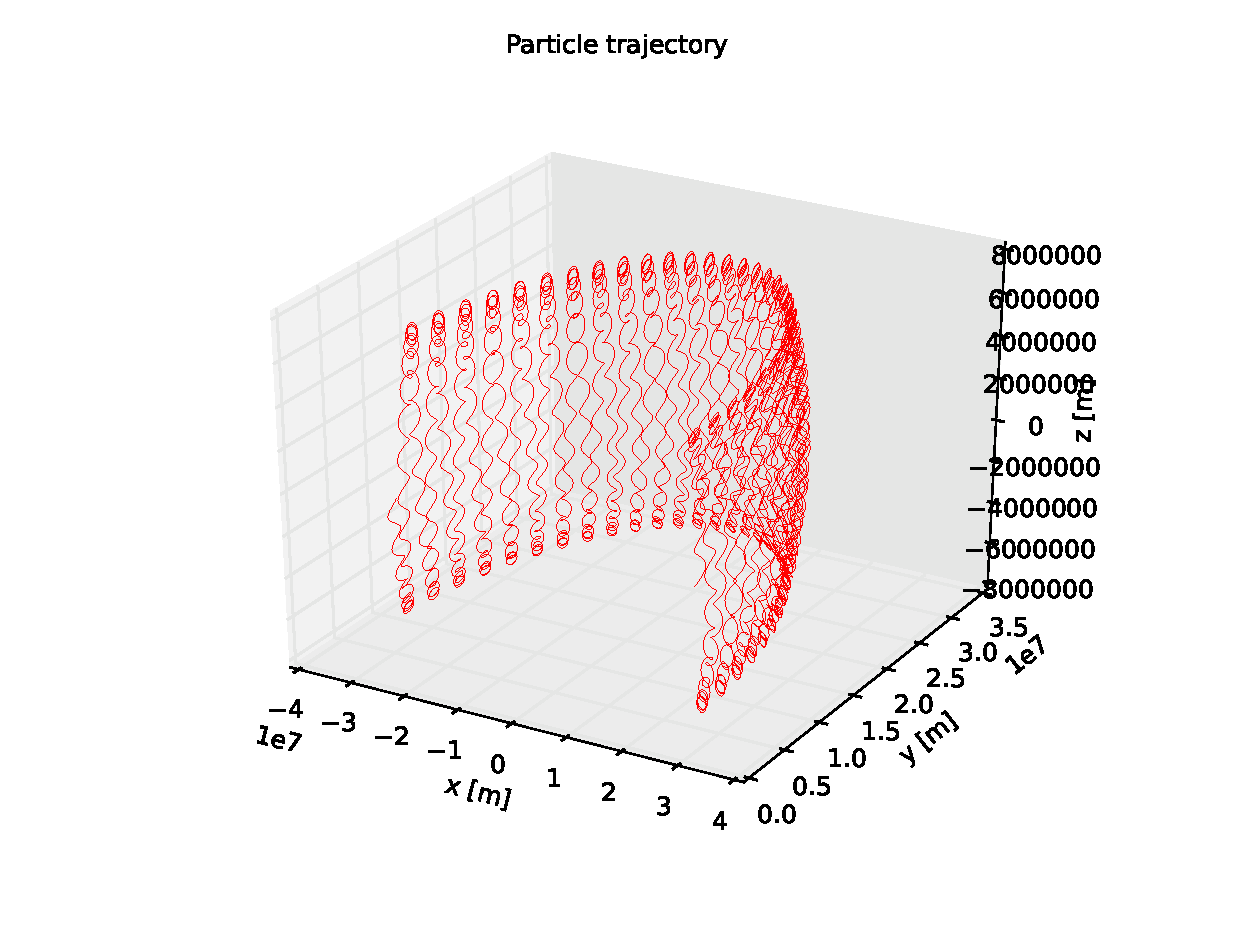
\includegraphics[width = \textwidth]{figures/rk4_3D_6_2}
      \end{subfigure}
      \begin{subfigure}{0.33\textwidth}
        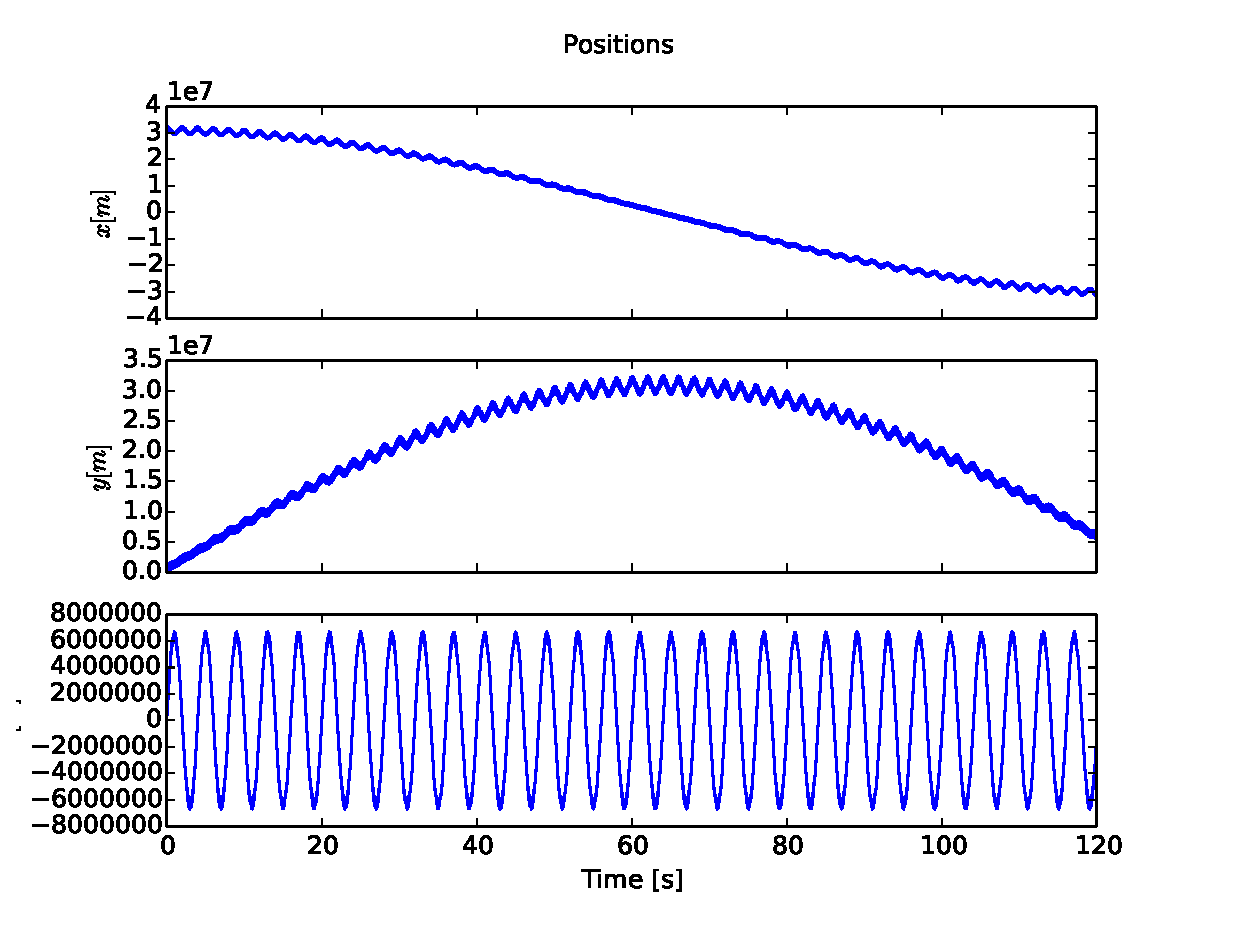
\includegraphics[width = \textwidth]{figures/rk4_xyz_6_2}
      \end{subfigure}
      \begin{subfigure}{0.33\textwidth}
        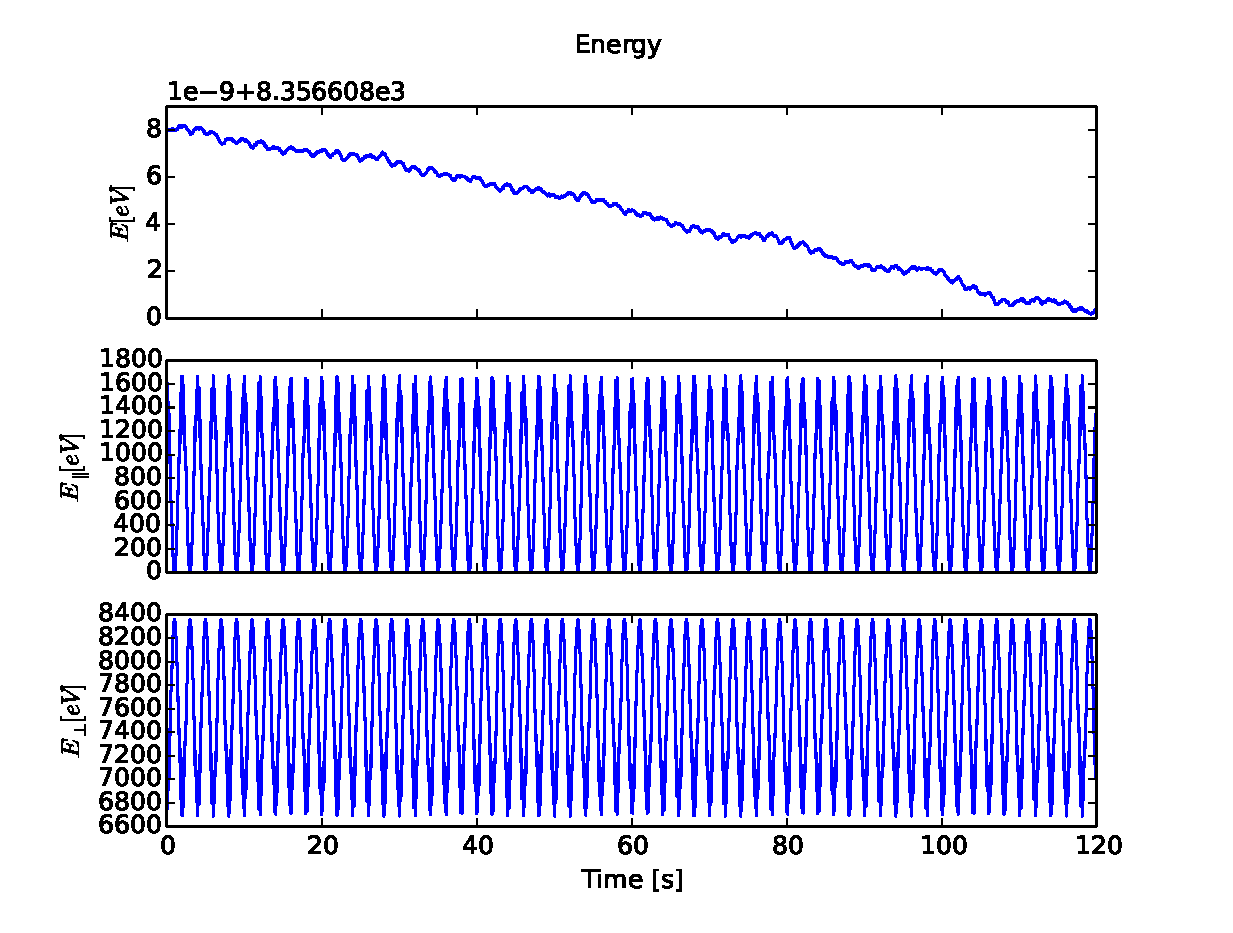
\includegraphics[width = \textwidth]{figures/rk4_E_6_2}
      \end{subfigure}
      \caption{The trajectory, positions and energy for an oxygen ion for with a \(\Delta t = 10^-2\), starting at \(v_0 = 10^5 \si{ms^{-1} }\).}
      \label{fig:results}
    \end{figure}

    In both the trajectory and the plot of the z-position we can clearly see that the particle is bouncing back and forth between then poles. There is also a drift in the eastward direction that can be seen most easily in the plot of the trajectory, but can also be seen as the x-coordinate is gradually decreasing and the y-coordinate is increasing. Since a magnetic field cannot do any work on a moving particle the total energy is conserved. When the particle due to the magnetic mirroring is losing the parallel velocity the perpendicular velocity is increasing so the total energy is conserved. 


    \subsubsection{Gyro period}
    Since the magnetic field is cylindrical symmetric, so let us use that and measure that as fast movements of the angle between the \(x-\) and \(y-\) coordinates. The gyration period will also change as it is dependent on \(|\va{B}|\), so the average is measured. For the run in \cref{fig:high_vel} with a high velocity an average gyration period of \( 0.155 \si{\second}\)was measured.

    \subsubsection{Bounce period}
    The particle will start by moving north compared with earth following the magnetic field lines, then as the magnetic field line density increases the parallel velocity will decrease. A static magnetic field does no work on a particle so the perpendicular velocity must increase. Since it will bounce between the north and south pole, the easiest method to measure it is to note how long time it takes between each time the particle crosses equator, \(z = 0\).

    The measurements in \cref{fig:high_vel} give a rough estimate of the bounce period of \( 4.0 \si{\second}\)

    \subsubsection{Drift period}
    The drift period is the time a particle trapped in earths magnetic dipole field takes to drift around earth. Since we know the \(x-\) and \(y-\)coordinates we can calculate the longitude of the particles position as \( \phi = \arctan{x/y} \). Then we can roughly say that \(\Delta \phi = \arctan(\Delta x / \Delta y) \).

    The measured drift period was measured in \cref{fig:high_vel} to be \(250 \si{\second}\).


\appendix
\section{Comments regarding the exercise}
      \begin{itemize}
            \item Parenthesis in Eq. 1 on the sheet is missing.
            \item I assume you mean the perpendicular and parallel \textit{kinetic} energy in part 2.
            \item Implemented RK4 instead, which worked much better, with a managable error, see \cref{sec:error}. So if you want them to analyze the energy, which has the plus that energy conservation be used as a test to see that the code is working correctly, RK4 is safer. It also has the perk that it runs decently with a much higher stepsize so the coding can be much more inefficient.
            \item The other option is to just use Eulers method and drop the part about the conserved energy. With the velocity, \(10^5\), the basic part of the trajectory is clearly visible and it shouldn't be to bothered by the increasing total energy before a whole drift period.
            \item I tried with the proposed velocity of \(10^6 \si{\meter\per\second}\) and the trajectory moved too fast between the bounces so the gyration was much harder to see. There is a figure of a trajactory in \cref{sec:high_vel}, showing it.
      \end{itemize}

\section{Error propagation RK4 vs Euler}
  \label{sec:error}
    \begin{figure}[ht]
      \begin{subfigure}{0.33\textwidth}
        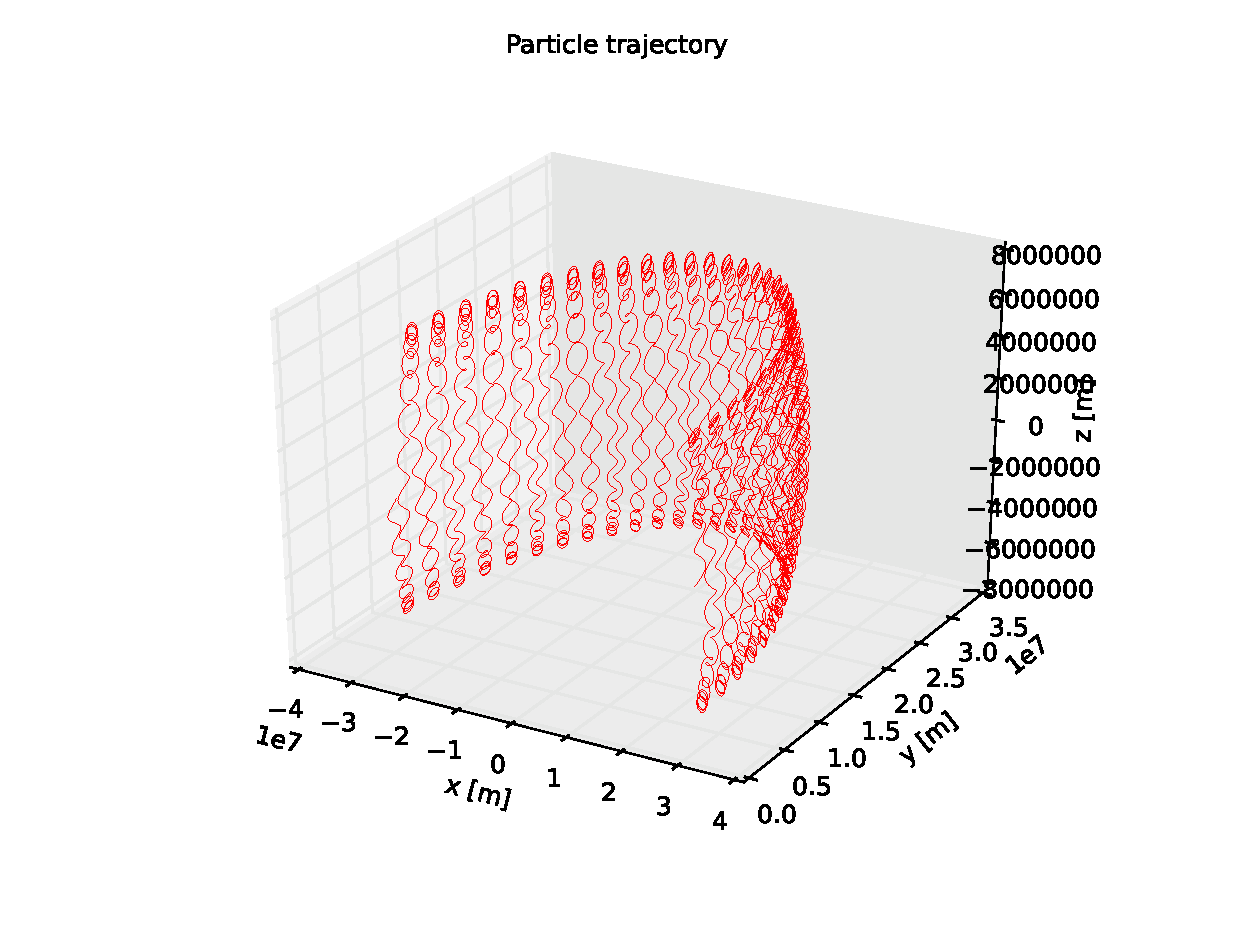
\includegraphics[width = \textwidth]{figures/rk4_3D_6_2}
      \end{subfigure}
      \begin{subfigure}{0.33\textwidth}
        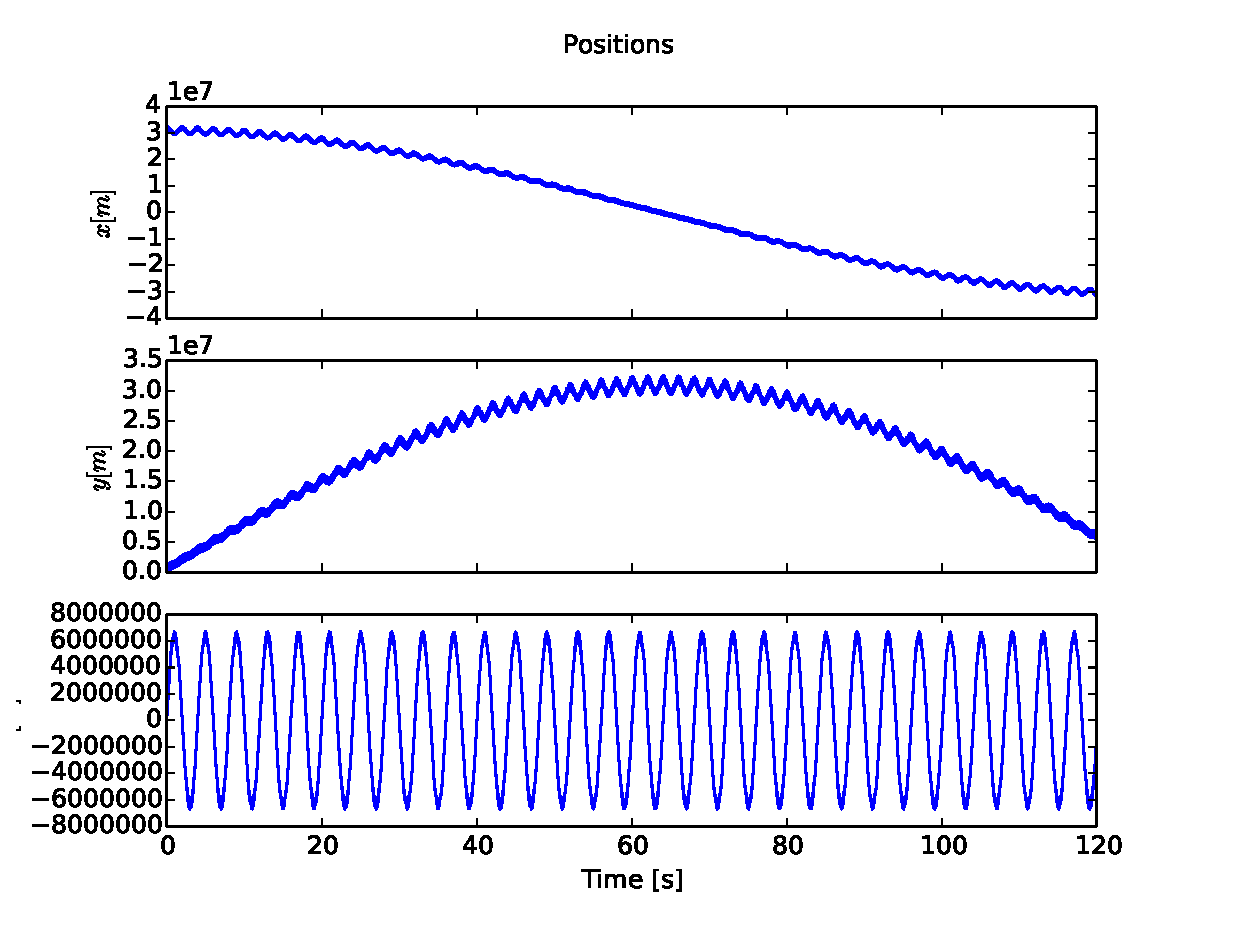
\includegraphics[width = \textwidth]{figures/rk4_xyz_6_2}
      \end{subfigure}
      \begin{subfigure}{0.33\textwidth}
        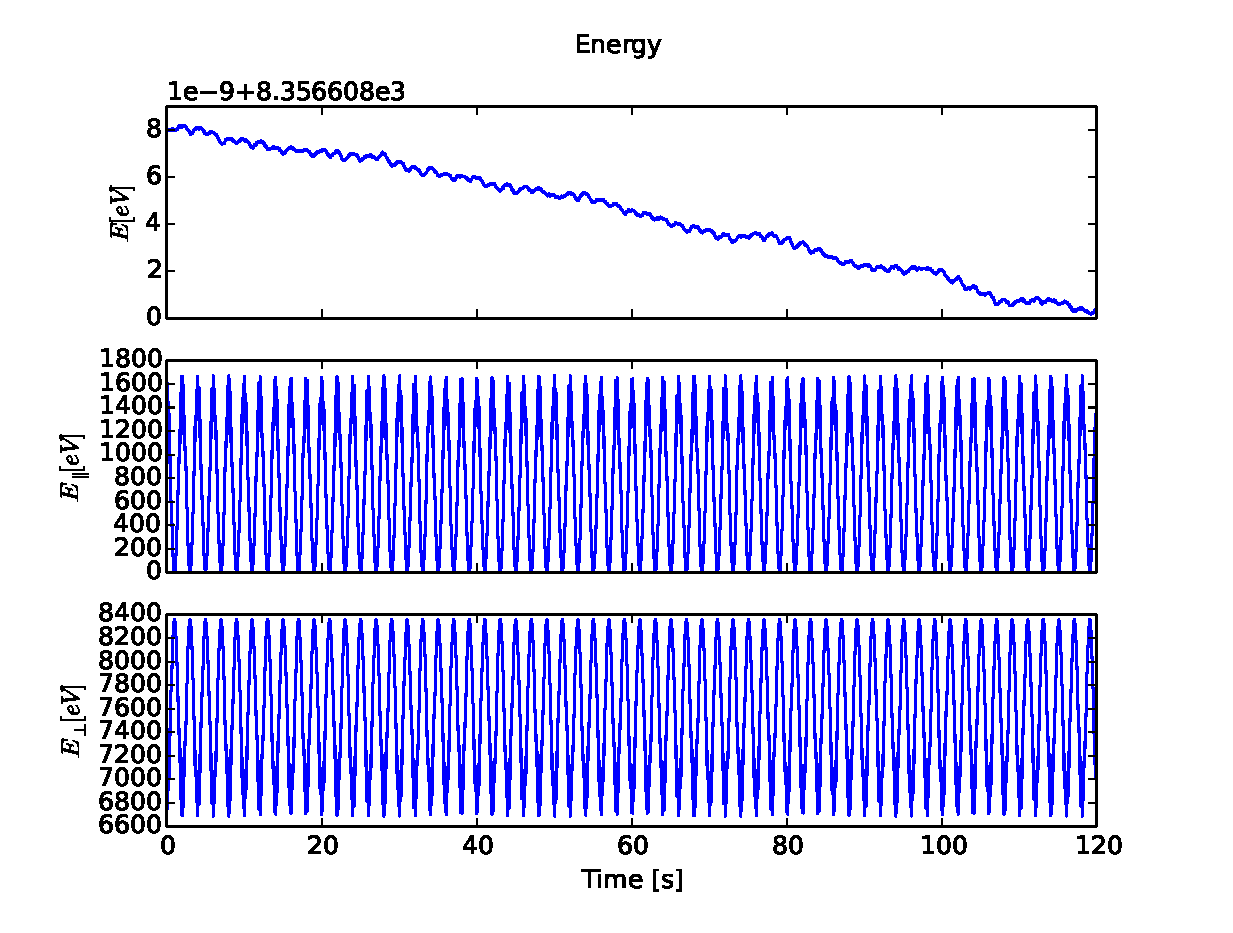
\includegraphics[width = \textwidth]{figures/rk4_E_6_2}
      \end{subfigure}
      \caption{The trajectory, positions and energy for an oxygen ion for with a \(\Delta t = 10^-2\), starting at \(v_0 = 10^5 \si{ms^{-1} }\).}
      \label{fig:results}
    \end{figure}

    

\section{ Trajectory high speed }
  \label{sec:high_vel}
    In \cref{fig:high_vel} is the trajectory with the high velocity of \(10^6 \si{\meter\per\second}\), with a pitch angle of \(25\si{\degree}\). The trajectory is gets very messy and I think a lower velocity is better so the gyration is clearly visible.

    \begin{figure}
      \centering 
      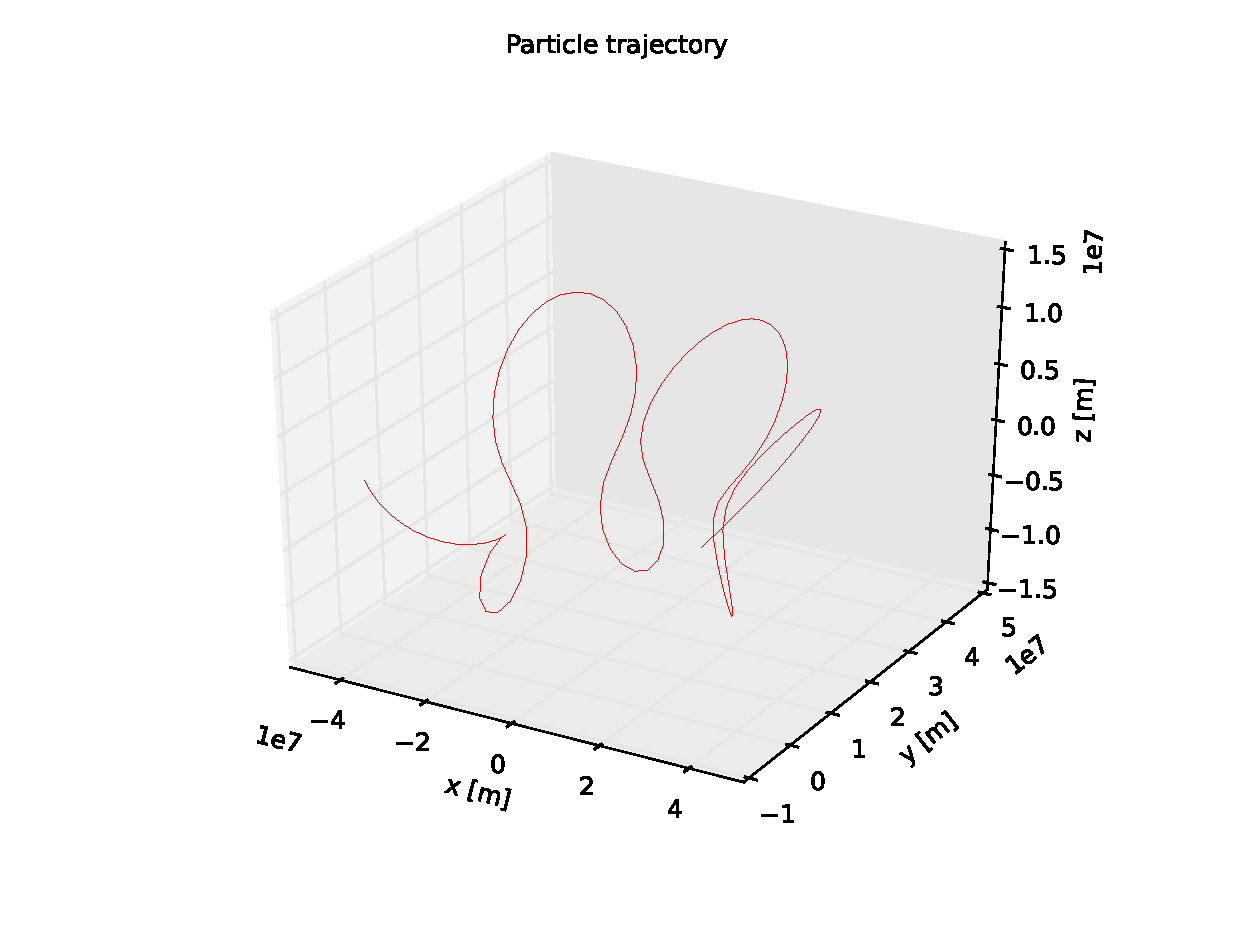
\includegraphics[width = 0.5\textwidth]{figures/rk4_3D_v6}
      \caption{The trajectory of an oxygen ion with an initial velocity of \(10^6 \si{\meter\per\second}\), with a pitch angle of \(25\si{\degree}\).}
      \label{fig:high_vel}
    \end{figure}




\section{Code}
  \label{sec:code}
  \lstinputlisting{../source/dipfield_rk4.py}

      

\end{document}